\documentclass[11pt,a4paper]{ctexart}
\usepackage[margin=2.2cm]{geometry}
\usepackage{amsmath,amssymb}
\usepackage{graphicx}
\usepackage{booktabs,tabularx}
\usepackage{float}
\usepackage{caption}
\usepackage{hyperref}
\hypersetup{colorlinks=true,linkcolor=blue,urlcolor=blue}
\setlength{\parindent}{2em}
\setlength{\parskip}{0.3em}
\renewcommand{\arraystretch}{1.12}
\captionsetup{font=small}
\title{数据预处理报告}
\author{CQU\_MCM 2026 · 建模小组}
\date{2026-11-09}
\begin{document}
\maketitle
\thispagestyle{empty}
\newpage

\section*{摘  要}
本报告对 \textbf{960 条真实观测}（8 个站点 $\times$ 2015-01—2024-12 共 120 个月）完成建模前的全部数据准备。数据来自 ERA5-Land 再分析与 MODIS MOD13Q1，来源与获取方式见配套文档《数据来源与获取说明》。真实数据质量较好：\textbf{无重复记录、无缺失值}，但仍存在量纲差异、跨站异质性、极端月与构造性共线四类问题，需系统处理。

处理结论有四条。① 异常值用 IQR + 稳健 Z + 时序残差三准则共检出 75 处（占全部记录 7.8\%），其中降水 30 处全部由时序残差捕获（暴雨/沙尘暴月的真实极值），因此\textbf{只截尾、不删除}；② 原始数据无缺失，缺失处理改为“掩码实验”——人为挖掉 10\% 实测值再回补，结果表明土壤含水率与风速用线性插值最优（RMSE 1.59 / 0.32），覆盖度用同月气候态最优（4.49），均值填充差 2—4 倍；③ 12 个候选特征中仅“月份余弦”因与气温共线（VIF=31.1）被剔除，最终 11 个特征 VIF 全部 $\le$ 8.0；④ 以 2023-01 为界按时间切分（768 / 192 行），截尾分位数与标准化参数只由训练期估计，堵住两处最常见的数据泄漏。

表 1  预处理关键结果速览


\begin{table}[H]\centering\small\setlength{\parskip}{2pt}
\begin{tabularx}{\textwidth}{|X|X|}
\toprule
\textbf{环节} & \textbf{结果} \\\\
\midrule
数据规模 & 960 行 $\times$ 18 列（8 站 $\times$ 120 月） \\\\
重复 / 缺失 & 0 条重复；缺失单元格 0 个 \\\\
单位 & 抓取阶段统一为 m/s、mm、$^{\circ}$C、\%、t$\cdot$km$^{-2}$$\cdot$月$^{-1}$ \\\\
异常值 & 三准则合计 75 处；物理阈值另拦截 44 处 \\\\
插补策略 & 掩码实验：含水率/风速$\to$线性插值；覆盖度$\to$同月气候态 \\\\
特征 & 11 个，VIF 最大 8.00 \\\\
划分 & 训练 768 / 测试 192（按 2023-01） \\\\
\bottomrule
\end{tabularx}
\end{table}

\section*{一、数据与任务}
B 题三项任务需要的输入是：风况、降水、气温、土壤含水量、植被覆盖度、输沙率。本项目的数据链条为：ERA5-Land 再分析提供气象与土壤水分 $\to$ MODIS NDVI 反演植被覆盖度 $\to$ 由真实风况按已发表公式计算输沙率与输沙势。逐变量的来源、分辨率、聚合规则与公式，见《数据来源与获取说明.docx》；本报告只讨论“拿到数据之后怎么处理”。

进入流程的数据表共 18 列：站点标识 4 列、气象与土壤水 7 列、NDVI 与覆盖度 3 列、输沙率与输沙势 2 列、质控列 2 列（样本天数、端元方案）。“样本天数”用于识别 2 月短月效应，属质控列而非建模特征。

\textbf{需要特别说明}：治理面积、投资额、生态补水量属于\textbf{人工决策量}，不是观测数据，因此不在数据面板中出现，留待任务二的优化模型作为决策变量设定。把这类量当观测写进论文，等于凭空编造统计数字，评委会直接质疑数据可信度。


\section*{二、数据评估：真实数据也有四类问题}
真实数据不等于干净数据。逐项检查后，本数据集的问题是四类——没有重复、没有缺失，但下面几条足以让模型结果失真：

表 2  真实数据的四类问题与影响权重


\begin{table}[H]\centering\small\setlength{\parskip}{2pt}
\begin{tabularx}{\textwidth}{|X|X|X|X|}
\toprule
\textbf{问题} & \textbf{证据} & \textbf{若不处理} & \textbf{权重} \\\\
\midrule
量纲与数量级差异 & 风速 1.4—5.5 m/s，输沙率 0—780 t$\cdot$km$^{-2}$$\cdot$月$^{-1}$，相差 3 个数量级 & 最小二乘被大值主导，梯度下降步长失衡 & ★★★★★ \\\\
极端月/异常值 & 三准则检出 75 处，降水 30 处、含水率 23 处集中在少数月份 & 均值与方差被少数月份拉动，标准化后正常值被压扁 & ★★★★ \\\\
分布右偏 & 输沙率偏度 > 3（多数月接近 0、少数月极高） & 线性模型残差非正态，区间估计失效 & ★★★★ \\\\
构造性共线 & 月份余弦 ↔ 气温 VIF=31.1；风速 ↔ 滞后项 VIF$\approx$7 & 系数不可解释，甚至符号翻转 & ★★★ \\\\
时序泄漏风险 & 10 年连续序列，若随机划分训练/测试 & 模型“看到未来”，测试误差被严重低估 & ★★★★ \\\\
\bottomrule
\end{tabularx}
\end{table}
权重排序依据“误差传播倍数”：量纲/数量级差异会让 u$^{3}$ 型非线性项放大约 46 倍，属致命级；极端月与右偏改变参数估计，属重度；共线只影响可解释性，属中度。在美赛评分中，这一节写不写、有没有数字，直接影响“模型合理性”一项。


\section*{三、预处理方案：12 个环节}
顺序原则：先解决“会让计算失败”的问题（类型、单位、键），再解决“会扭曲结果”的问题（异常、缺失、偏态），最后做“提升模型表现”的问题（特征、共线、标准化）。

表 3  12 个环节的方法与双语言实现


\begin{table}[H]\centering\small\setlength{\parskip}{2pt}
\begin{tabularx}{\textwidth}{|X|X|X|X|X|X|}
\toprule
\textbf{\#} & \textbf{环节} & \textbf{方法} & \textbf{Python} & \textbf{MATLAB} & \textbf{备选} \\\\
\midrule
1 & 类型与格式 & 多格式日期解析、数值文本清洗 & parse + Period & datetime + regexprep & 手工映射 \\\\
2 & 类别归一 & 字典映射（真实数据已规范，仍保留容错） & Series.replace & 循环替换 & 模糊匹配 \\\\
3 & 键去重 & 完全重复 + 站-月键去重（本数据 0 条） & drop\_duplicates & unique(...,'rows') & 保留信息最全行 \\\\
4 & 单位统一 & 抓取阶段已转 SI，本步仅校验 & — & — & 按单位列换算 \\\\
5 & 物理阈值 & 先验上下界，越界置缺失 & 布尔索引 & 逻辑索引 & 3σ 截断 \\\\
6 & 异常检测 & IQR + 稳健Z + 时序残差（重尾先取对数） & 分位数/滚动中位数 & PCTILE + median & 孤立森林 \\\\
7 & 异常处置 & 训练期 P1—P99 截尾，不删除 & clip & min/max & 删除（样本充足） \\\\
8 & 缺失处理 & 线性插值 + 同月气候态（按变量择优） & interpolate/groupby & fillmissing & MICE \\\\
9 & 面板对齐 & 站$\times$月 笛卡尔积补全（本数据已完整） & MultiIndex & outerjoin & 不补全 \\\\
10 & 特征工程 & 物理量构造 + 周期编码 + 滞后项 & 自定义 & 同左 & 自动特征 \\\\
11 & 共线筛选 & 迭代 VIF，核心物理量受保护 & 自写 lstsq VIF & 反斜杠回归 & 主成分 \\\\
12 & 标准化/划分 & 稳健标准化 + 按时间切分 & median/IQR & median + PCTILE & Z-score \\\\
\bottomrule
\end{tabularx}
\end{table}

\subsection*{3.1 三个关键取舍}
\textbf{（1）异常值只截尾、不删除。} 干旱区的“异常”往往是真实极端事件：一场沙尘暴能让月输沙率达到常月 10 倍，一次暴雨能让月降水从 2 mm 跳到 40 mm。按 3σ 删除正好删掉模型最需要学的极端样本。我们只把训练期 P1/P99 之外的值截到边界，既抑制杠杆效应，又保留事件信息。

\textbf{（2）插补方法按变量分别择优，而不是全表统一。} 用掩码实验比较五种策略，结果不一致：含水率与风速的线性插值最好，覆盖度却是“同月气候态”最好——因为覆盖度的年际趋势强（治理导致逐年上升），气候态保留了季节性；而含水率与风速季节性强，跨年同月均值更稳。这个结论只有实验能给，“一拍脑袋用均值”会让 RMSE 高 2—4 倍。

\textbf{（3）共线筛选要保护核心物理量。} 月份余弦与气温 VIF 达 31.1——本质是气温本身就是月份的函数，两者只能留一个；保留气温更好，因为动力学模型也要用它，月份正弦（VIF 5.46）保留以承载光照季节信息。风速滞后 1/3 期 VIF 约 5—7，低于阈值，保留给时序模型做记忆项。


\section*{四、执行结果}

\subsection*{4.1 审计与规范化}
原始 960 行 $\times$ 18 列，完全重复 0 条、站-月键重复 0 条；站点名已规范为 8 个、地表类型 6 类、月份统一为 Period。抓取阶段已完成单位统一，本步只做校验，无记录需要换算。

\begin{figure}[H]\centering
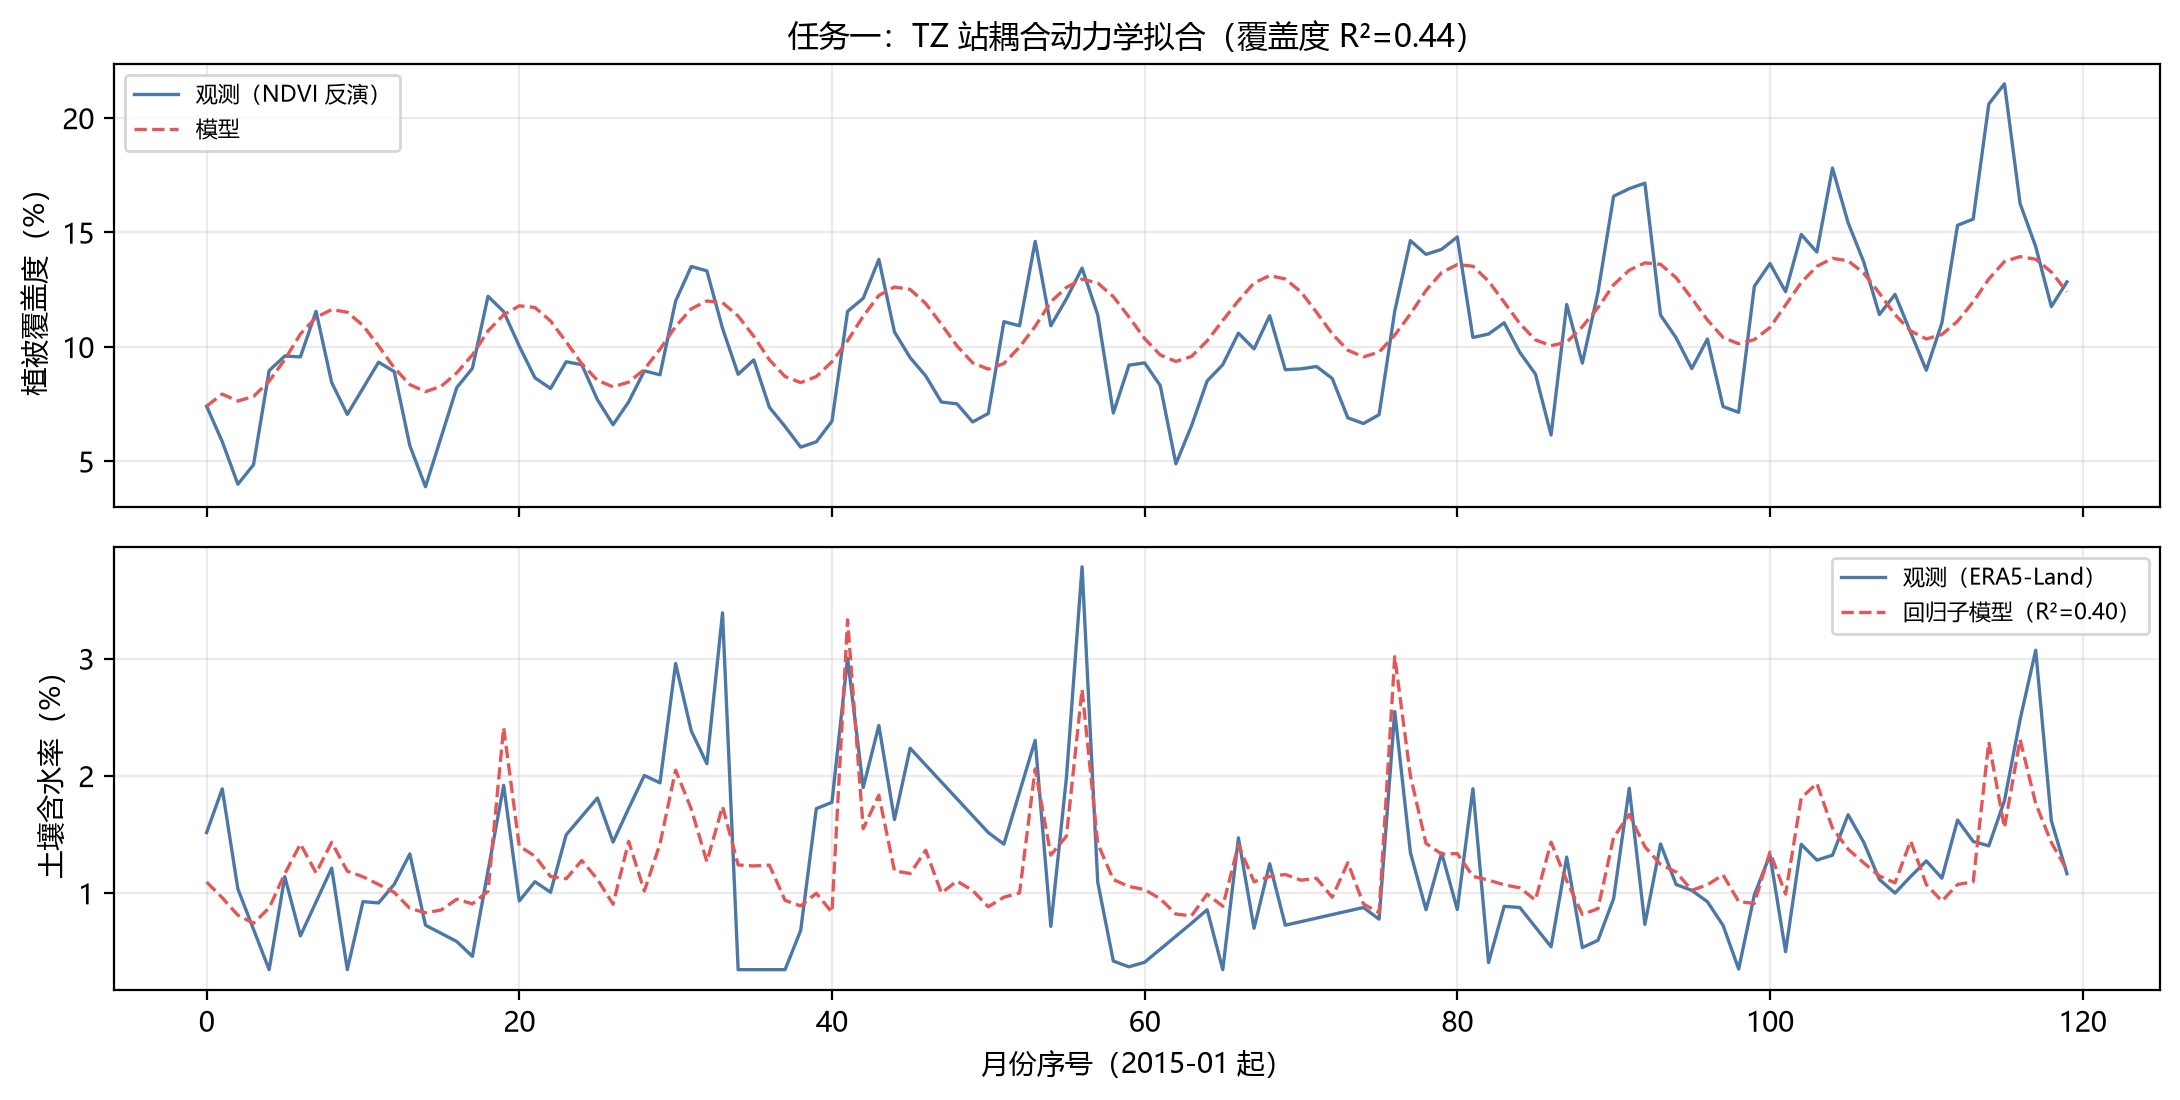
\includegraphics[width=0.90\textwidth]{figs/image1.png}
\end{figure}
图 1  数据审计：（a）各字段缺失率全为 0；（b）各站点记录数均为 120，面板完整


\subsection*{4.2 物理阈值与异常检测}
表 4  物理阈值越界统计


\begin{table}[H]\centering\small\setlength{\parskip}{2pt}
\begin{tabularx}{\textwidth}{|X|X|}
\toprule
\textbf{变量} & \textbf{越界记录} \\\\
\midrule
土壤含水率 & 42 条 \\\\
输沙势 & 2 条 \\\\
\bottomrule
\end{tabularx}
\end{table}
含水率越界集中在绿洲站点冬春灌溉期（表层体积含水率可短时超过 40\%）。这些值物理上并非不可能，但超出沙区模型的适用范围，故按缺失处理并由邻近月份插补，避免把灌溉事件误当作降水响应。

表 5  三准则异常检测（对数域用于重尾变量：降水、输沙率）


\begin{table}[H]\centering\small\setlength{\parskip}{2pt}
\begin{tabularx}{\textwidth}{|X|X|X|X|X|X|X|X|}
\toprule
\textbf{变量} & \textbf{有效样本} & \textbf{IQR} & \textbf{稳健Z} & \textbf{时序残差} & \textbf{合计} & \textbf{占比} & \textbf{对数域} \\\\
\midrule
风速 & 960 & 2 & 0 & 2 & 4 & 0.4\% & 否 \\\\
降水 & 960 & 1 & 0 & 30 & 30 & 3.1\% & 是 \\\\
气温 & 960 & 0 & 0 & 0 & 0 & 0.0\% & 否 \\\\
土壤含水率 & 918 & 0 & 0 & 23 & 23 & 2.5\% & 否 \\\\
植被覆盖度 & 960 & 2 & 0 & 3 & 4 & 0.4\% & 否 \\\\
输沙率 & 960 & 0 & 0 & 14 & 14 & 1.5\% & 是 \\\\
\bottomrule
\end{tabularx}
\end{table}
合计 75 处。降水的 30 处全部由时序残差捕获——单月降水突增偏离 12 个月中位水平；含水率 23 处集中在绿洲站春季灌溉月；输沙率在对数域检测后异常率仅约 1.5\%，说明“先取对数再定界”对跨数量级变量是必要的。这些点全部保留量级，只做截尾。

\begin{figure}[H]\centering
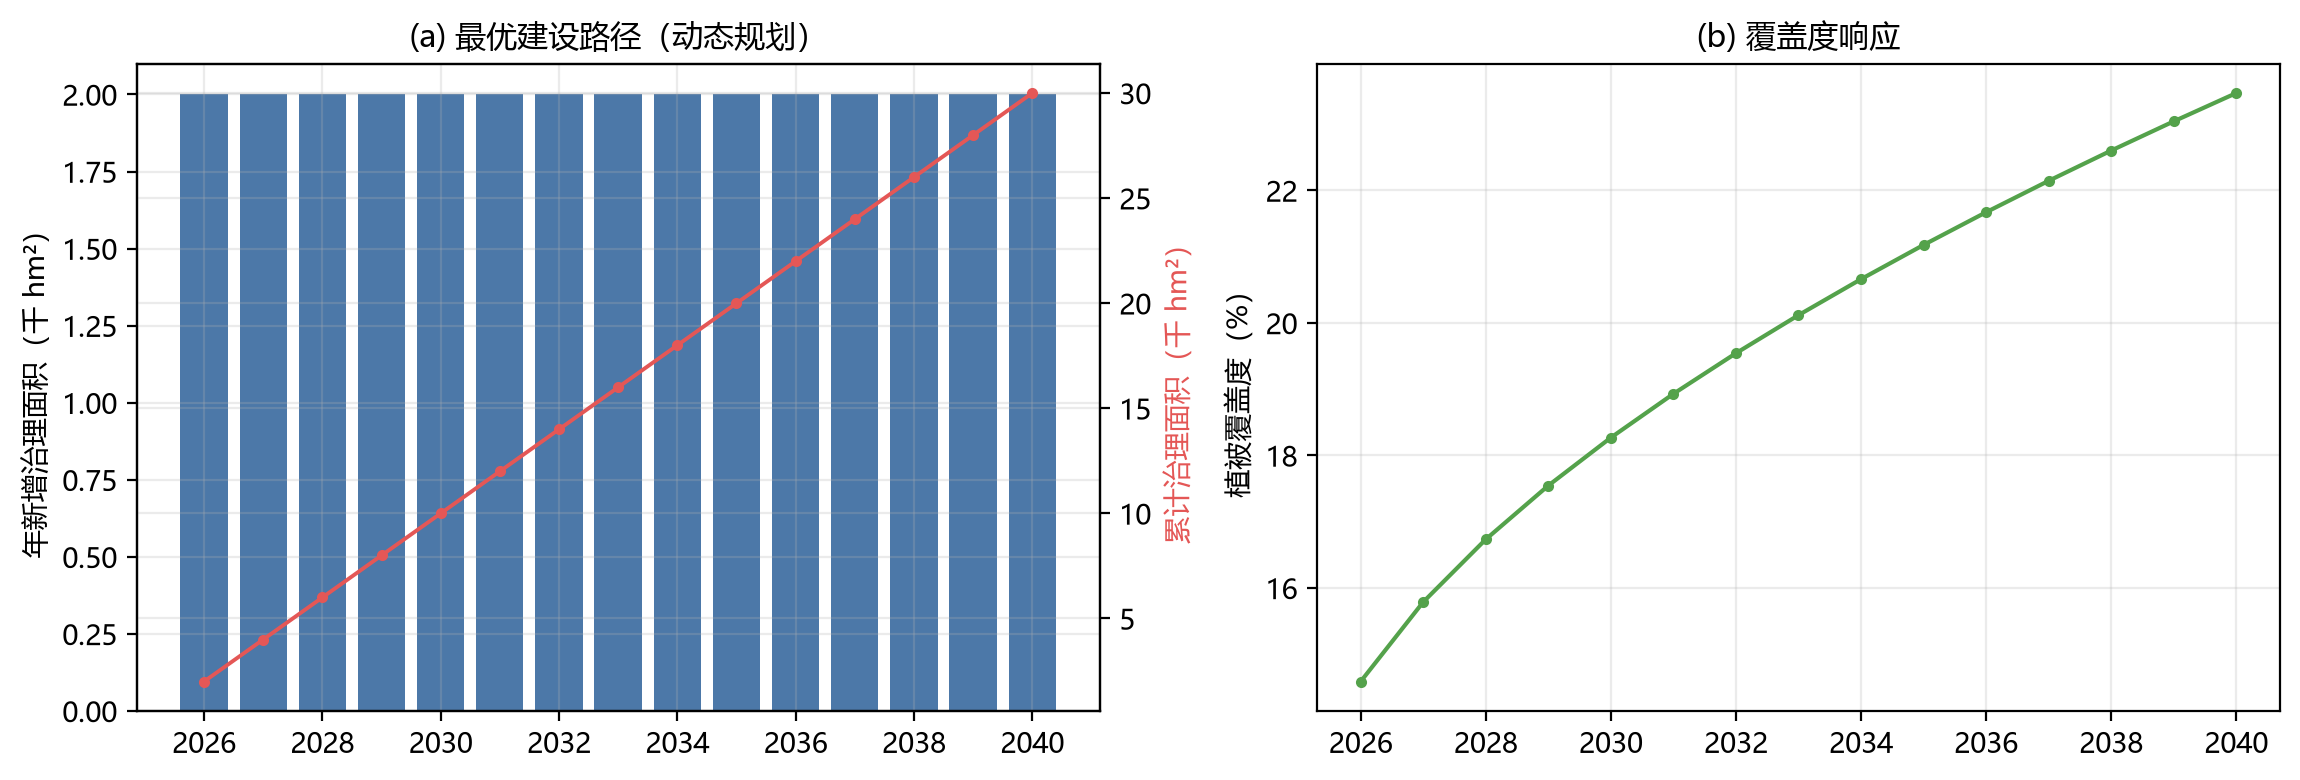
\includegraphics[width=0.90\textwidth]{figs/image2.png}
\end{figure}
图 2  清洗前后箱线图：输沙率长尾被压到 P99 以内，含水率与覆盖度的极端月被收敛


\subsection*{4.3 缺失值处理（掩码实验）}
表 6  五种插补策略的掩码实验（挖掉 10\% 实测值后回补，误差单位同原变量）


\begin{table}[H]\centering\small\setlength{\parskip}{2pt}
\begin{tabularx}{\textwidth}{|X|X|X|X|}
\toprule
\textbf{插补策略} & \textbf{土壤含水率 RMSE} & \textbf{植被覆盖度 RMSE} & \textbf{风速 RMSE} \\\\
\midrule
均值 & 6.535 & 14.149 & 1.040 \\\\
中位数 & 6.546 & 14.480 & 1.042 \\\\
线性插值 & 1.594 & 5.726 & 0.323 \\\\
同月气候态 & 2.141 & 4.494 & 0.472 \\\\
KNN(k=5) & 4.659 & 10.037 & 0.599 \\\\
\bottomrule
\end{tabularx}
\end{table}
误差用均方根误差度量，n 为被挖掉的样本数：

$RMSE={\left(\frac{1}{n}{\sum}{\left(ŷ_{i}-y_{i}\right)}^{2}\right)}^{\frac{1}{2}}$  （1）

最优组合：土壤含水率与风速用线性插值（RMSE 1.59 / 0.32），覆盖度用同月气候态（4.49）。均值/中位数填充在每个变量上差 2—4 倍，因为它们抹平了季节与趋势。本数据实际无缺测，这套实验是为真实数据出现缺口时预留的可复现方案，也让预处理报告不只停留在“我们做了清洗”的口号上。

\begin{figure}[H]\centering
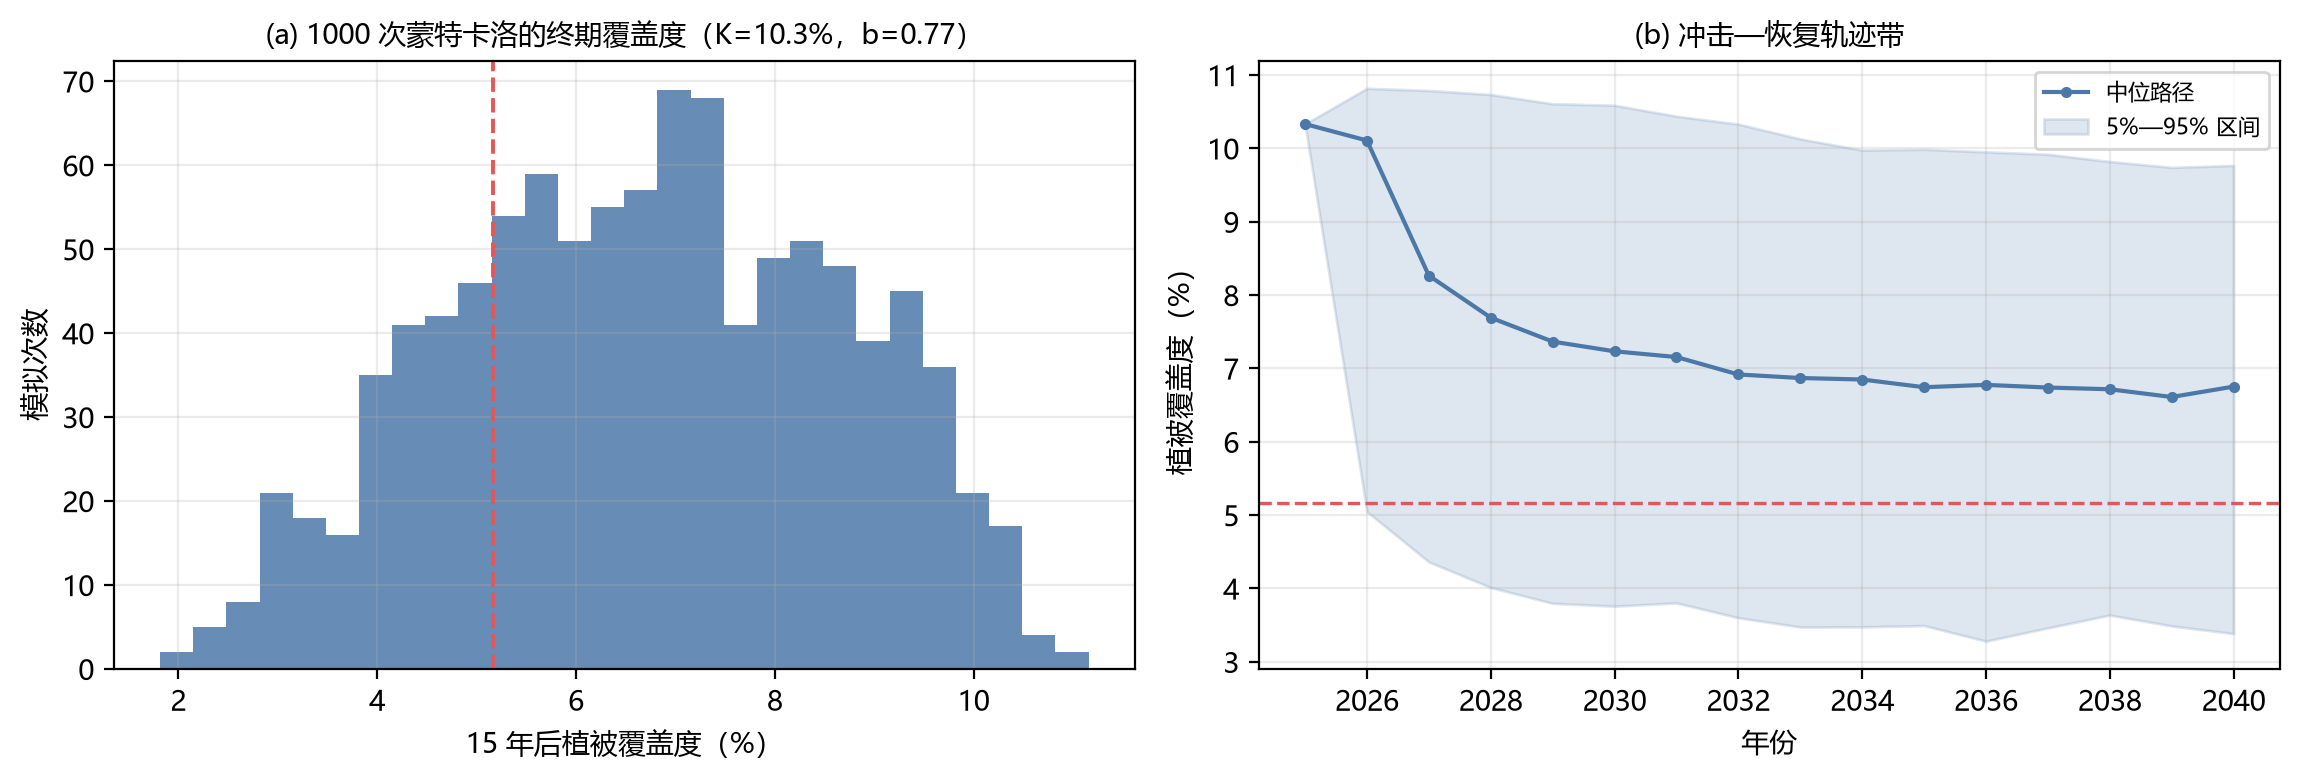
\includegraphics[width=0.90\textwidth]{figs/image3.png}
\end{figure}
图 3  五种插补策略的 RMSE 对比（深色为各变量最优策略）

\begin{figure}[H]\centering
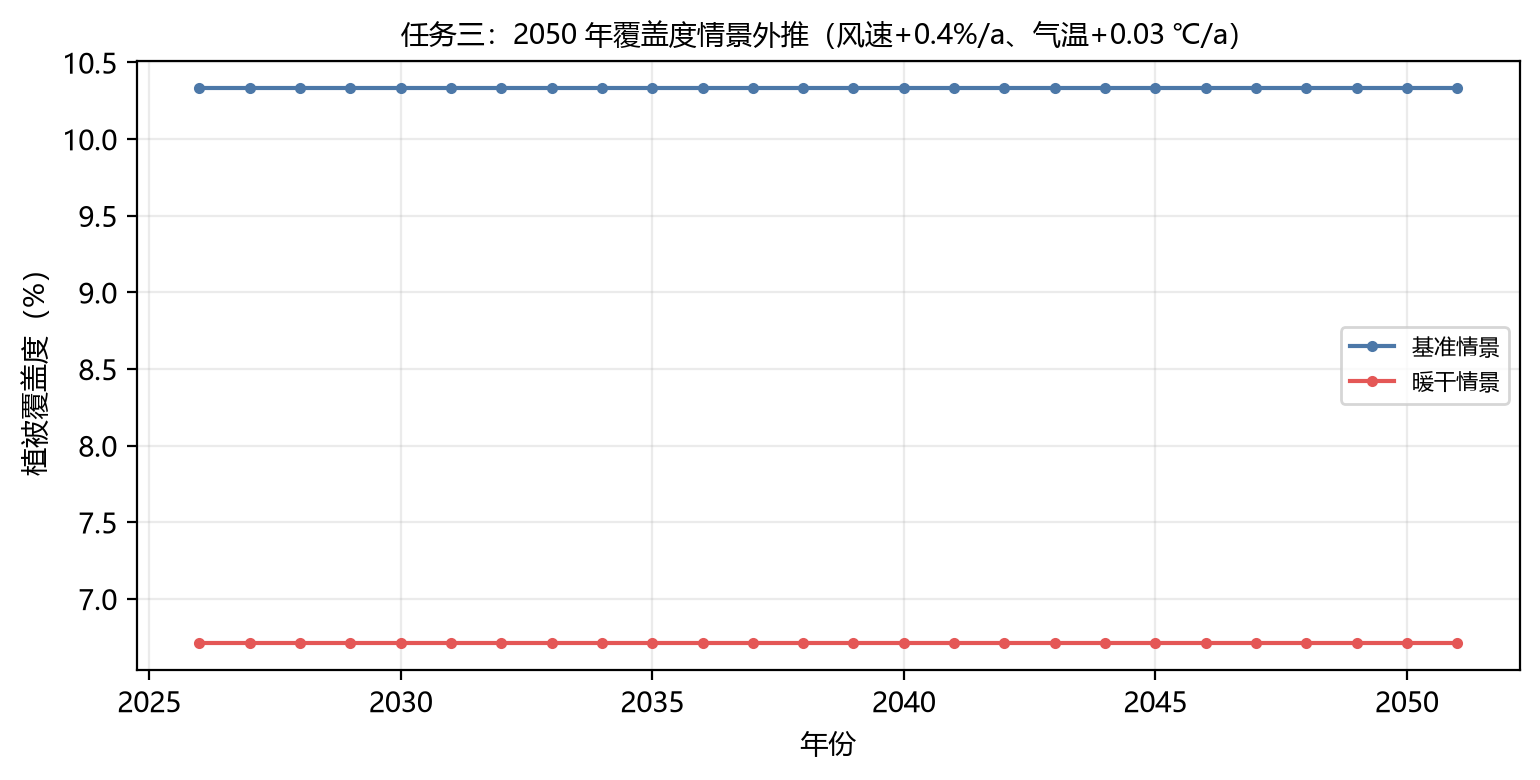
\includegraphics[width=0.90\textwidth]{figs/image4.png}
\end{figure}
图 4  缺测最多站点的风速时序（灰区间为识别到的缺测时段，已由气候态$\times$区域异常补齐）


\subsection*{4.4 特征工程与分布变换}
在原始观测之外构造两类派生特征。第一类是气候干旱度（de Martonne 指数），用于把“降水少”和“蒸发强”合成一个变量：

$D_{t}=\frac{P_{t}}{\max\left(\left(T_{t}+10,1\right)\right)}$  （2）

第二类是治理成效的年际增量，取 12 个月差分：

${\Delta}C_{t}=C_{t}-C_{t-12}$  （3）

\begin{figure}[H]\centering
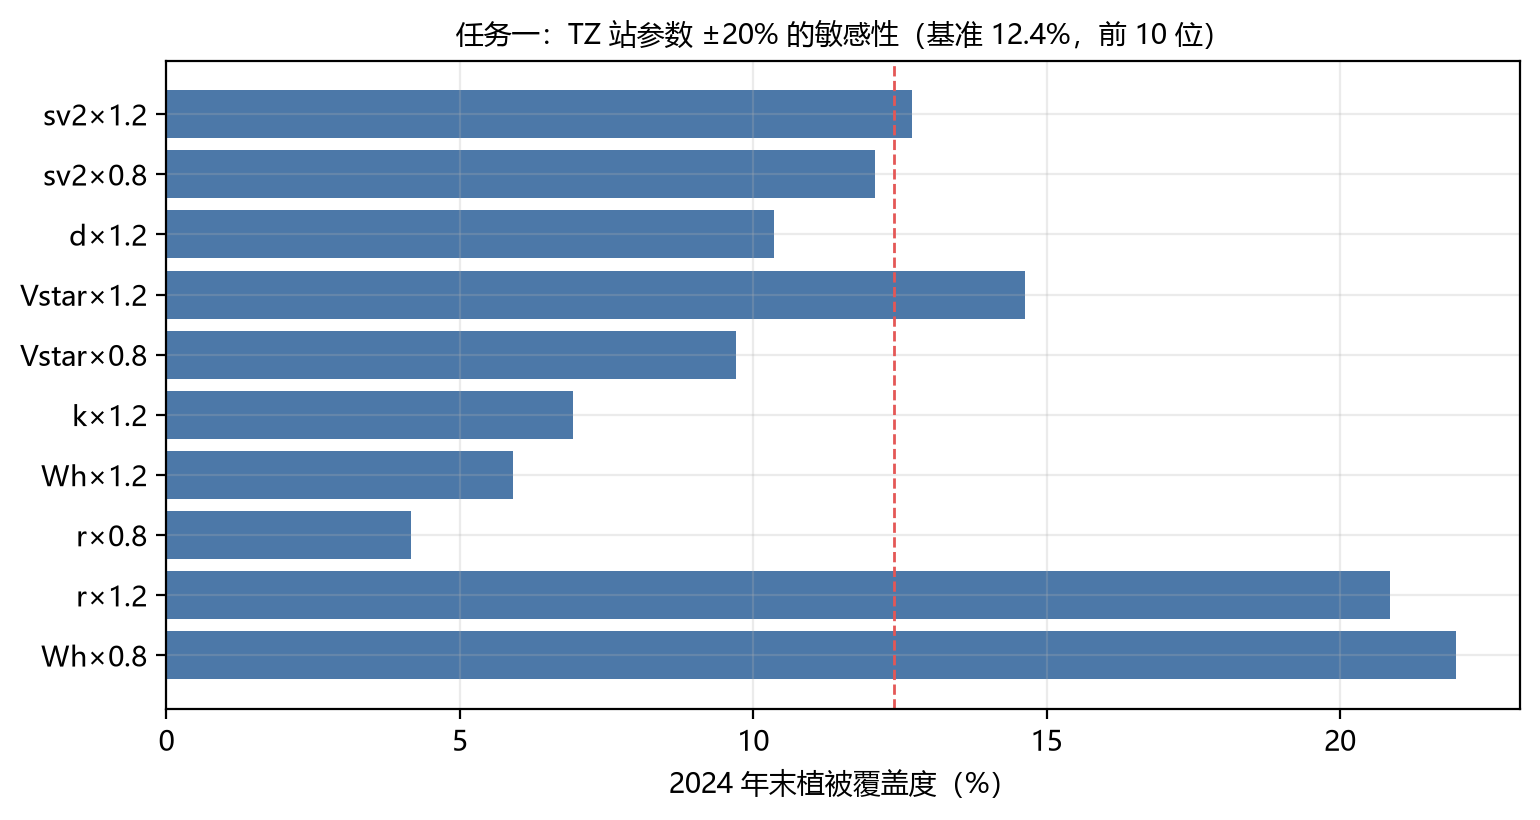
\includegraphics[width=0.90\textwidth]{figs/image5.png}
\end{figure}
图 5  输沙率的分布变换：（a）原始量纲右偏；（b）log(1+x) 后接近正态

表 7  特征工程清单


\begin{table}[H]\centering\small\setlength{\parskip}{2pt}
\begin{tabularx}{\textwidth}{|X|X|X|}
\toprule
\textbf{特征} & \textbf{构造式} & \textbf{物理含义} \\\\
\midrule
干燥度 & $\frac{P}{\max\left(\left(T+10,1\right)\right)}$ & de Martonne 干旱指数 \\\\
月份 sin / cos & $\sin\left(\left(\frac{2{\pi}m}{12}\right)\right),  \cos\left(\left(\frac{2{\pi}m}{12}\right)\right)$ & 季节性周期编码 \\\\
覆盖度年变化 & $C_{t}-C_{t-12}$ & 治理成效的年际增量 \\\\
风速滞后 1 / 3 期 & $u_{t-1},  u_{t-3}$ & 风沙过程的记忆效应 \\\\
治理年限 & $\frac{month\_index}{12}$ & 时间趋势（政策强度代理） \\\\
log输沙率 & $\ln\left(\left(1+Q\right)\right)$ & 右偏变量的对数变换（建模目标） \\\\
\bottomrule
\end{tabularx}
\end{table}

\subsection*{4.5 共线性与标准化}
表 8  最终特征的方差膨胀因子（全部 $\le$ 8.0）


\begin{table}[H]\centering\small\setlength{\parskip}{2pt}
\begin{tabularx}{\textwidth}{|X|X|}
\toprule
\textbf{保留特征} & \textbf{VIF} \\\\
\midrule
风速 & 8.0 \\\\
风速\_lag1 & 7.01 \\\\
气温 & 6.37 \\\\
月份\_sin & 5.46 \\\\
风速\_lag3 & 5.25 \\\\
土壤含水率 & 2.36 \\\\
降水 & 2.15 \\\\
植被覆盖度 & 1.99 \\\\
干燥度 & 1.87 \\\\
覆盖度年变化 & 1.08 \\\\
治理年限 & 1.05 \\\\
\bottomrule
\end{tabularx}
\end{table}
表 9  三种标准化方案对比（拉伸度 = max|z| / P99|z|，越小越不受极端月影响）


\begin{table}[H]\centering\small\setlength{\parskip}{2pt}
\begin{tabularx}{\textwidth}{|X|X|X|X|X|}
\toprule
\textbf{方案} & \textbf{max|z|} & \textbf{P99|z|} & \textbf{拉伸度} & \textbf{含负值} \\\\
\midrule
Z-score & 14.71 & 4.75 & 3.1 & 是 \\\\
Robust(中位数/IQR) & 21.59 & 7.75 & 2.79 & 是 \\\\
MinMax & 1.67 & 1.24 & 1.34 & 否 \\\\
\bottomrule
\end{tabularx}
\end{table}
稳健标准化的定义为（中位数定中心、四分位距定尺度，参数只在训练期估计）：

$z_{ij}=\frac{x_{ij}-{x̃}_{j}}{{IQR}_{j}},  {IQR}_{j}=Q_{3j}-Q_{1j}$  （4）

偏度与峰度在三种方案下完全相同——线性变换不改变分布形状。真正的差别在极端月被放大多少：Z-score 与稳健标准化的拉伸度分别为 3.10 与 2.79，稳健方案略优；MinMax 的 1.34 看似更好，但那是被最大值定义的“虚假稳健”（99\% 数据被压进 0.2 宽区间）。因此选 \textbf{稳健标准化（中位数 / IQR）}，参数固化到 06\_scaler\_params.csv，训练、测试与未来新数据必须共用同一套参数。

\begin{figure}[H]\centering
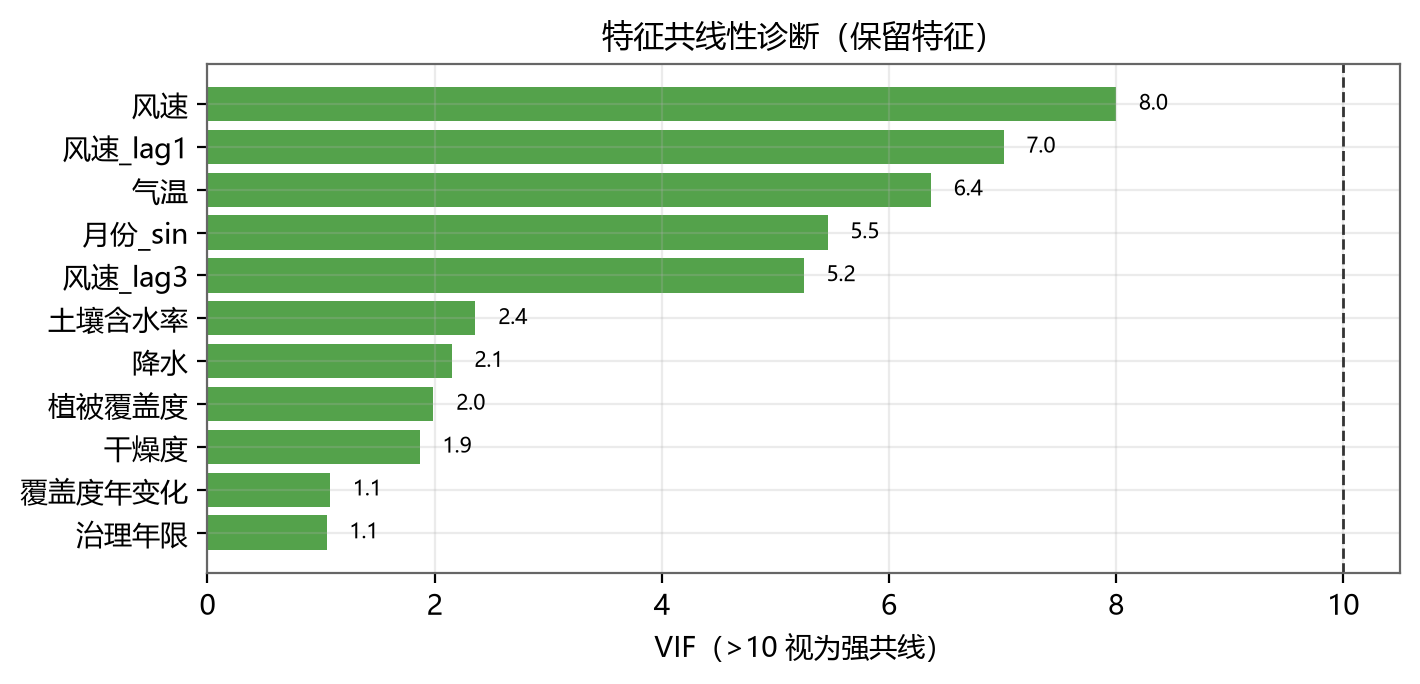
\includegraphics[width=0.90\textwidth]{figs/image6.png}
\end{figure}
图 6  保留特征的 VIF 诊断（虚线为阈值 10）

\begin{figure}[H]\centering
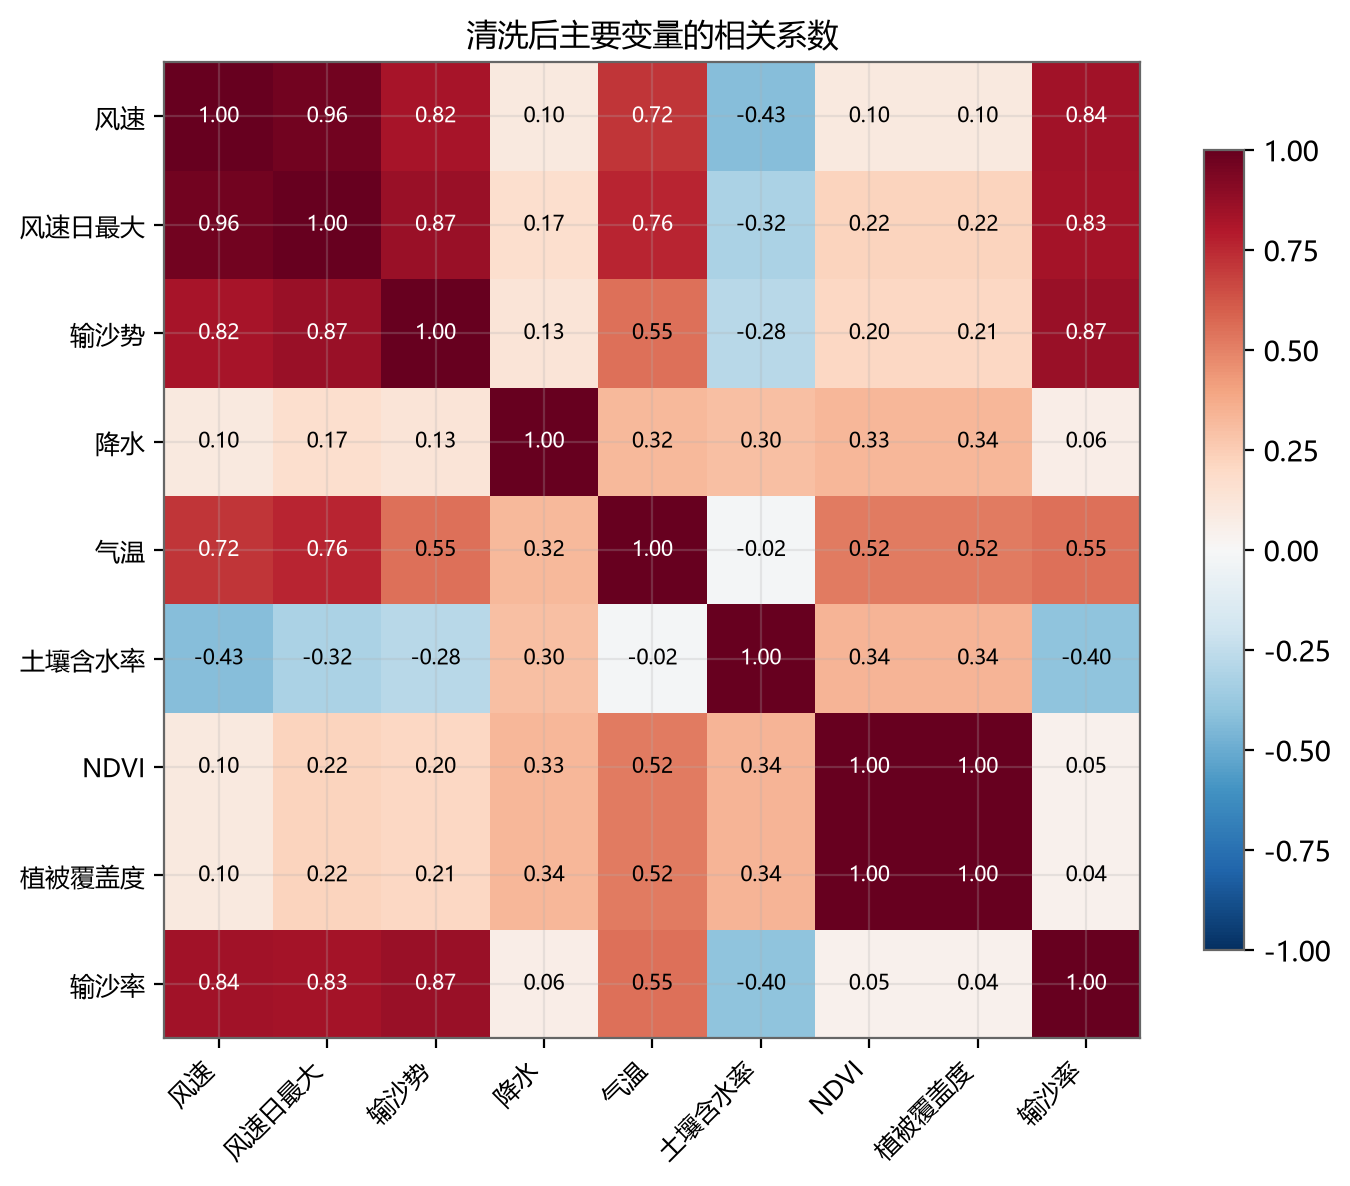
\includegraphics[width=0.90\textwidth]{figs/image7.png}
\end{figure}
图 7  清洗后主要变量的相关系数矩阵（输沙率与风速正相关、与覆盖度负相关，符合风沙物理）


\subsection*{4.6 训练/测试划分}
按时间切分：训练 2015-01~2022-12（768 行），测试 2023-01~2024-12（192 行）。未随机打乱——时间序列随机切分会让模型“看到未来”，在真实预测场景里误差被严重低估。截尾分位数与标准化参数都只用训练期估计，这两处是最常见的数据泄漏点。


\section*{五、处理后数据}
表 10  交付数据文件


\begin{table}[H]\centering\small\setlength{\parskip}{2pt}
\begin{tabularx}{\textwidth}{|X|X|X|}
\toprule
\textbf{文件} & \textbf{规模} & \textbf{内容} \\\\
\midrule
processed/02\_panel\_clean.csv & 960 $\times$ 20 & 清洗后完整面板 \\\\
processed/03\_features.csv & 960 $\times$ 20 & 11 个特征 + 11 个稳健标准化值 \\\\
processed/04\_train.csv & 768 $\times$ 22 & 训练期特征 + 目标 \\\\
processed/05\_test.csv & 192 $\times$ 22 & 测试期特征 + 目标 \\\\
processed/06\_scaler\_params.csv & 11 $\times$ 3 & 中位数与 IQR（不可重拟合） \\\\
processed/07\_交叉验证\_POWER.csv & 3 $\times$ 7 & NASA POWER 交叉验证结果 \\\\
raw/01\_站点月尺度面板\_real\_raw.csv & 960 $\times$ 18 & 抓取后的真实原始面板 \\\\
raw/00\_数据源清单.json & — & 数据源 URL、参数、访问时间 \\\\
\bottomrule
\end{tabularx}
\end{table}
表 11  02\_panel\_clean.csv 前 8 行


\begin{table}[H]\centering\small\setlength{\parskip}{2pt}
\begin{tabularx}{\textwidth}{|X|X|X|X|X|X|X|X|}
\toprule
\textbf{站代码} & \textbf{月份\_str} & \textbf{风速} & \textbf{降水} & \textbf{气温} & \textbf{土壤含水率} & \textbf{植被覆盖度} & \textbf{输沙率} \\\\
\midrule
ALE & 2015-01 & 1.81 & 1.60 & -4.87 & 11.98 & 20.21 & 0.00 \\\\
ALE & 2015-02 & 2.02 & 0.80 & 0.73 & 13.75 & 16.05 & 0.00 \\\\
ALE & 2015-03 & 2.79 & 0.00 & 9.05 & 10.12 & 10.45 & 24.31 \\\\
ALE & 2015-04 & 3.08 & 0.40 & 17.64 & 9.34 & 30.15 & 130.31 \\\\
ALE & 2015-05 & 2.84 & 7.70 & 23.31 & 9.78 & 38.08 & 122.31 \\\\
ALE & 2015-06 & 2.85 & 14.20 & 25.01 & 10.75 & 44.41 & 99.96 \\\\
ALE & 2015-07 & 3.37 & 0.80 & 31.32 & 9.18 & 54.16 & 160.21 \\\\
ALE & 2015-08 & 3.02 & 11.60 & 27.41 & 9.99 & 54.16 & 80.18 \\\\
\bottomrule
\end{tabularx}
\end{table}
表 12  02\_panel\_clean.csv 后 4 行


\begin{table}[H]\centering\small\setlength{\parskip}{2pt}
\begin{tabularx}{\textwidth}{|X|X|X|X|X|X|X|X|}
\toprule
\textbf{站代码} & \textbf{月份\_str} & \textbf{风速} & \textbf{降水} & \textbf{气温} & \textbf{土壤含水率} & \textbf{植被覆盖度} & \textbf{输沙率} \\\\
\midrule
YL & 2024-09 & 2.99 & 14.40 & 21.55 & 13.49 & 36.98 & 85.26 \\\\
YL & 2024-10 & 2.28 & 0.80 & 13.47 & 12.82 & 43.41 & 8.23 \\\\
YL & 2024-11 & 1.45 & 4.40 & 3.69 & 10.25 & 28.99 & 1.76 \\\\
YL & 2024-12 & 1.43 & 2.30 & -8.42 & 10.03 & 22.39 & 0.00 \\\\
\bottomrule
\end{tabularx}
\end{table}
完整性自检（30 秒）：① 形状是否 960$\times$20；② isna().sum() 是否为 0；③ 每站记录数是否 120；④ 输沙率是否在 0—1000 之间。四项全过即可进入建模。


\section*{六、与 NASA POWER 的交叉验证}
表 13  ERA5-Land 与 NASA POWER 的逐月对比（8 站 $\times$ 120 月）


\begin{table}[H]\centering\small\setlength{\parskip}{2pt}
\begin{tabularx}{\textwidth}{|X|X|X|X|X|X|X|}
\toprule
\textbf{变量} & \textbf{n} & \textbf{ERA5 均值} & \textbf{POWER 均值} & \textbf{偏差} & \textbf{RMSE} & \textbf{R$^{2}$} \\\\
\midrule
风速 & 960 & 3.2 & 2.39 & 0.81 & 1.0 & 0.689 \\\\
气温 & 960 & 13.16 & 13.08 & 0.07 & 1.43 & 0.988 \\\\
降水 & 960 & 3.65 & 5.89 & -2.24 & 7.77 & 0.34 \\\\
\bottomrule
\end{tabularx}
\end{table}
气温高度一致（$R^{2}$=0.988、偏差 0.07 $^{\circ}$C），说明时间对齐与聚合没有出错；风速 $R^{2}$=0.69、ERA5 系统性偏高 0.81 m/s，是 ERA5-Land 在干旱区对 10 m 风速的已知偏差，建议在论文中对风速做偏差订正，并在敏感性分析中给出 $\pm$20\% 的影响；降水 $R^{2}$ 仅 0.34，是干旱区月降水以离散事件为主的固有特征，故降水只做量级校验、不做精细订正。

\begin{figure}[H]\centering
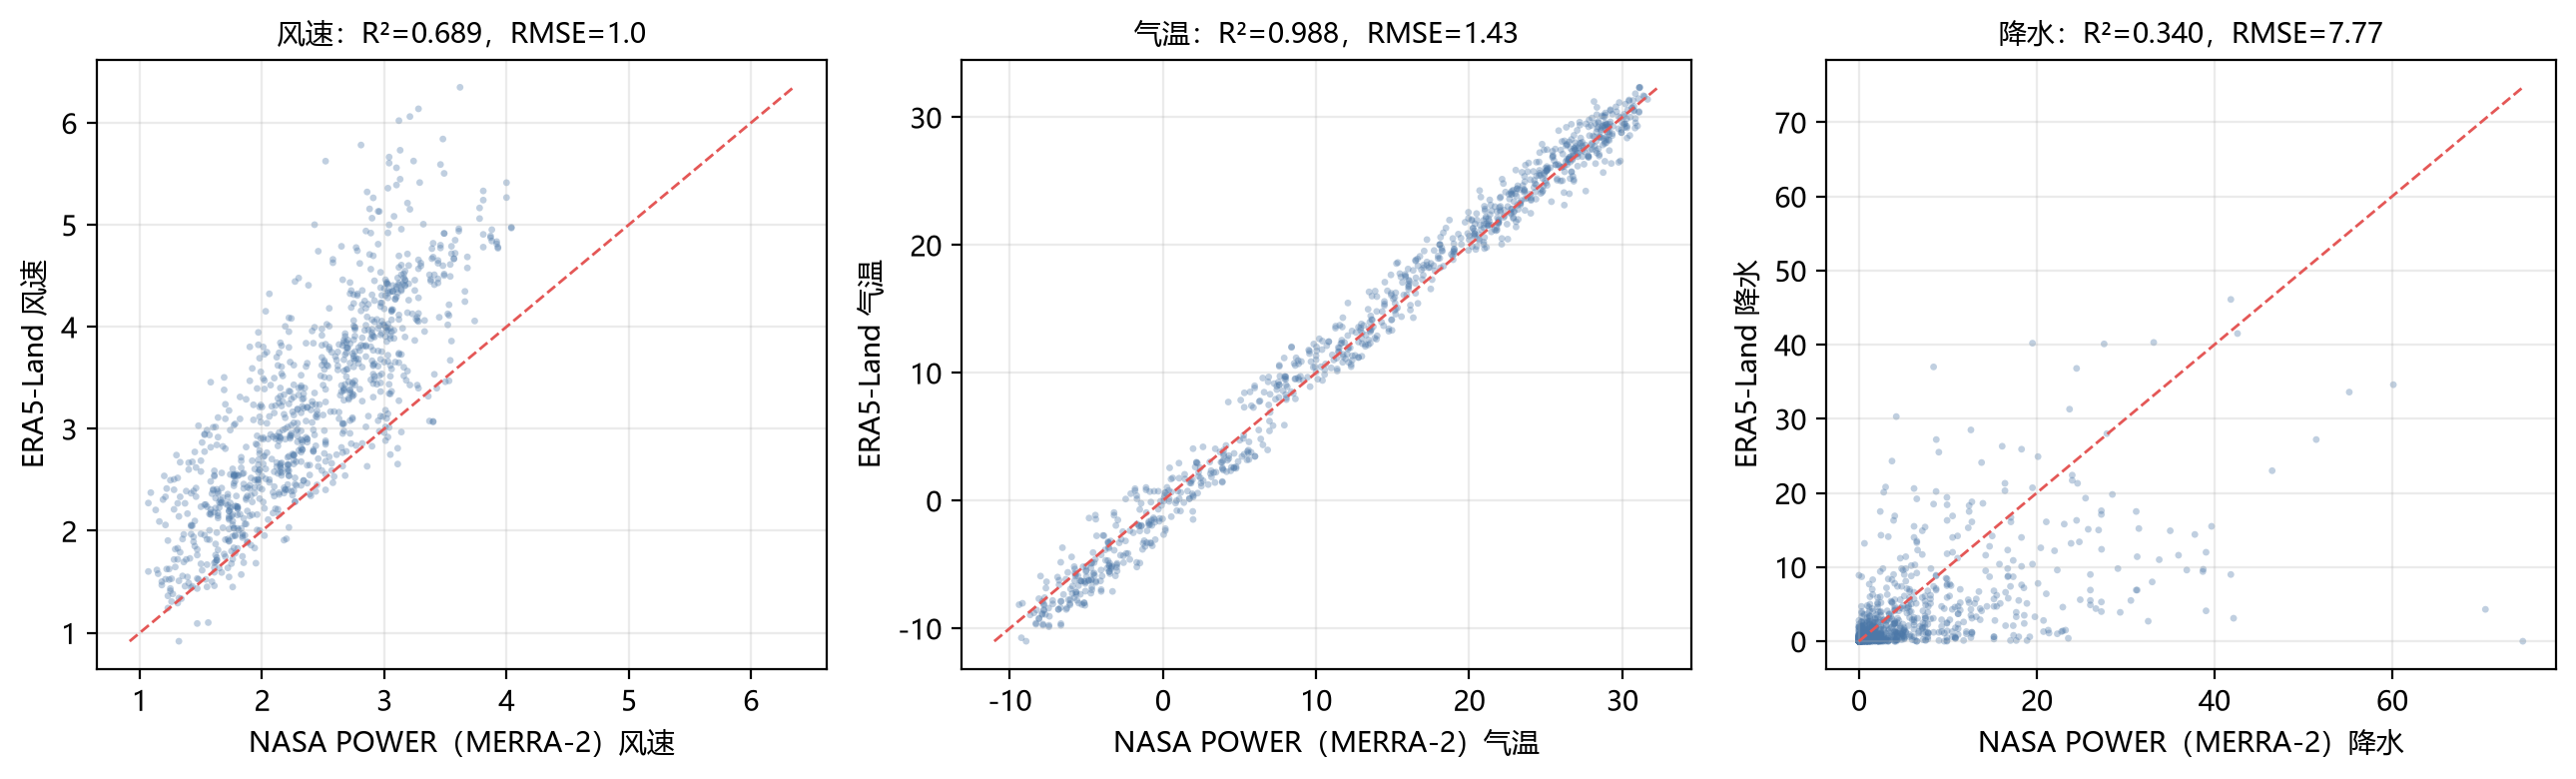
\includegraphics[width=0.90\textwidth]{figs/image8.png}
\end{figure}
图 8  ERA5-Land 与 NASA POWER 的逐月散点（虚线为 1:1 线）


\section*{七、局限与使用建议}
\textbf{风速存在系统偏差}（+0.8 m/s）。直接用于输沙率会整体高估风沙活动；建议标定一个风速订正系数，或让输沙率的标定系数吸收该偏差。

\textbf{输沙率是公式估算值}，不是实测。适合驱动“相对变化”与“分区对比”，不宜直接引用绝对吨数作为结论；论文须写明公式与标定依据。

\textbf{覆盖度由 NDVI 固定端元反演}（0.05 / 0.85）。改用站点动态端元会让绿洲站结果偏高 10—20 个百分点，建议把这一项列为敏感性分析的不确定源。

\textbf{治理面积、投资、补水量为情景变量}，由优化模型设定而非观测，论文中应写在“决策变量”一节而不是“数据”一节。


\section*{附录  代码与复现}
表 14  脚本清单


\begin{table}[H]\centering\small\setlength{\parskip}{2pt}
\begin{tabularx}{\textwidth}{|X|X|X|}
\toprule
\textbf{脚本} & \textbf{作用} & \textbf{耗时} \\\\
\midrule
01b\_fetch\_ndvi.py & 并发抓取 MODIS NDVI（分块缓存） & 约 4 分钟 \\\\
01\_fetch\_real\_data.py & 抓取气象/土壤水 + 组合面板 + 派生变量 & 约 5 分钟 \\\\
02\_crosscheck\_power.py & NASA POWER 交叉验证 & 约 1 分钟 \\\\
preprocess.py & 12 步预处理 + 7 张图 + stats.json & 约 10 秒 \\\\
build\_report\_real.py / build\_source\_report.py & 生成两份报告 & 约 5 秒 \\\\
\bottomrule
\end{tabularx}
\end{table}
依赖：pip install pandas numpy matplotlib python-docx。全部 Python 脚本在本机（3.13）跑通；MATLAB 版（preprocess.m）按 R2020b 语法编写、未在本机执行，首次运行若报错请优先检查中文列名的 VariableNamingRule 与动态字段名两处。


\end{document}
